%%%%%%%%%%%%%%%%%%%%%%%%%%%%%%%%%%%%%%%%%%%%%%%%%%%%%%%%%%%%%%%%%%%%%%%%%%%%%%%%%%%
%% This project aims to create the UFC template for presentation.                %%
%% author: Maurício Moreira Neto - Doctoral student in Computer Science (MDCC)   %%
%% contacts:                                                                     %%
%%    e-mail: maumneto@ufc.br                                                    %%
%%    linktree: https://linktr.ee/maumneto                                       %%
%%%%%%%%%%%%%%%%%%%%%%%%%%%%%%%%%%%%%%%%%%%%%%%%%%%%%%%%%%%%%%%%%%%%%%%%%%%%%%%%%%%
\documentclass{libs/ufc_format}
% Inserting the preamble file with the packages
%%%%%%%%%%%%%%%%%%%%%%%%%%%%%%%%%%%%%%%%%%%%%%%%%%%%%%%%%%%%%%%%%%%%%
%% This file contains the packages that can be used in the beamer. %%
%%%%%%%%%%%%%%%%%%%%%%%%%%%%%%%%%%%%%%%%%%%%%%%%%%%%%%%%%%%%%%%%%%%%%
% Package to fonts family
\usepackage[T1]{fontenc}
% Package to accentuation
\usepackage[utf8]{inputenc}
% Package to Portuguese language
\usepackage[brazil]{babel}
% Package to Figures
\usepackage{graphicx}
% Package to the colors
\usepackage{color}
% Package to the colors
\usepackage{xcolor}
% Packages to math symbols and expressions
\usepackage{amsfonts, amssymb, amsmath}
% Package to multiple lines and columns in table
\usepackage{multirow, array} 
% Package to create pseudo-code
% For more detail of this package: http://linorg.usp.br/CTAN/macros/latex/contrib/algorithm2e/doc/algorithm2e.pdf
\usepackage{algorithm2e}
% Package to insert code
\usepackage{listings} 
\usepackage{keyval}
% Package to justify text
\usepackage[document]{ragged2e}
% Package to manage the bibliography
\usepackage[backend=biber, style=numeric, sorting=none]{biblatex}
% Package to facilities quotations
\usepackage{csquotes}
% Package to use multicols
\usepackage{multicol}


%% On my own
\newcommand{\aspas}[1]{``#1''}

\usepackage{booktabs}
\usepackage{graphicx}
% Inserting the references file
\bibliography{references.bib}

% Title
\title[Aprendizado Estatístico em Dados Longitudinais]{\huge\textbf{Análise Completa do estudo de depressão de Riesby e do Crescimento de Árvores Sitka Spruce.}}
% Subtitle
\subtitle{}
% Author of the presentation
\author{Cícero Hitzschky}
% Institute's Name
\institute[UFC]{
    % email for contact
    \normalsize{\email{cicero.hitzschky@alu.ufc.br}}
    \newline
    % Department Name
    \department{Departamento de Estatística e Matemática Aplicada}
    \newline
    % university name
    \ufc
}
% date of the presentation
\date{\today}


%%%%%%%%%%%%%%%%%%%%%%%%%%%%%%%%%%%%%%%%%%%%%%%%%%%%%%%%%%%%%%%%%%%%%%%%%%%%%%%%%%
%% Start Document of the Presentation                                           %%               
%%%%%%%%%%%%%%%%%%%%%%%%%%%%%%%%%%%%%%%%%%%%%%%%%%%%%%%%%%%%%%%%%%%%%%%%%%%%%%%%%%
\begin{document}
% insert the code style
%%%%%%%%%%%%%%%%%%%%%%%%%%%%%%%%%%%%%%%%%%%%%%%%%%%%%%%%%%%%%%%%%%%%%%%%%%%%%%%%%%%
%% This file contains the style of the codes show in slides.                     %%
%% The package used is listings, but it possible to used others.                 %%
%%%%%%%%%%%%%%%%%%%%%%%%%%%%%%%%%%%%%%%%%%%%%%%%%%%%%%%%%%%%%%%%%%%%%%%%%%%%%%%%%%%

% color used in the code style
\definecolor{codegreen}{rgb}{0,0.6,0}
\definecolor{codegray}{rgb}{0.5,0.5,0.5}
\definecolor{codepurple}{rgb}{0.58,0,0.82}
\definecolor{codebackground}{rgb}{0.95,0.95,0.92}

% style of the code!
\lstdefinestyle{codestyle}{
    backgroundcolor=\color{codebackground},   
    commentstyle=\color{codegreen},
    keywordstyle=\color{magenta},
    numberstyle=\tiny\color{codegray},
    stringstyle=\color{codepurple},
    basicstyle=\ttfamily\footnotesize,
    frame=single,
    breakatwhitespace=false,         
    breaklines=true,                 
    captionpos=b,                    
    keepspaces=true,                 
    numbers=left,                    
    numbersep=5pt,                  
    showspaces=false,                
    showstringspaces=false,
    showtabs=false,                  
    tabsize=2,
    title=\lstname 
}

\lstset{style=codestyle}


%% ---------------------------------------------------------------------------
% First frame (with tile, subtitle, ...)
\begin{frame}{}
    \maketitle
\end{frame}

%% ---------------------------------------------------------------------------
% Second frame
\begin{frame}{Sumário}
    \begin{multicols}{2}
        \tableofcontents
    \end{multicols}
\end{frame}

%% ---------------------------------------------------------------------------
% This presentation is separated by sections and subsections
\section{Dataset Riesby}
\subsection{Desenho do Estudo}
\begin{frame}{Dataset Riesby}
    \begin{block}{Sobre o conjunto de dados}
    	\begin{itemize}
    		\justifying
    		\item O dataset Riesby representa um ensaio clínico psiquiátrico longitudinal descrito em Reisby et al. (1977) para tratamento de depressão.
    		\item O estudo focou na relação longitudinal entre os níveis plasmáticos de imipramina (IMI) e desipramina (DMI) e a resposta clínica em 66 pacientes internados com depressão é a mudança nas pontuações de depressão semana a semana.
    		\item Como a imipramina se biotransforma no metabólito ativo desmetilimipramina (ou desipramina), a medição da desipramina também foi feita neste estudo.
    	\end{itemize}
    \end{block}
\end{frame}

\begin{frame}{Desenho do Estudo}
	\begin{block}{Fase Inicial}
		Período de Placebo 
	\end{block}
	\begin{block}{Tratamento}
		Doses de 225mg/dia de imipramina por 4 semanas.
	\end{block}
	\begin{block}{Avaliação}
		Escala de classificação de depressão de Hamilton (Hamilton, 1960).
	\end{block}
	\begin{block}{Medições}
		Nível plasmático de imipramina (IMI) e seu metabólito desipramina (DMI) medidos no final de cada semana de tratamento.
	\end{block}
\end{frame}

\begin{frame}{Desenho do Estudo}
	\begin{block}{Coleta de dados}
		\begin{itemize}
			\item Sexo
			\item Diagnóstico de Depressão: Endógena ou Reativa (Não endógena).
		\end{itemize}
	\end{block}
\end{frame}

\begin{frame}{Desenho do Estudo}
	\begin{block}{Número de Participantes}
		Um total de 66 indivíduos sendo a variação por semana dada por:
		\begin{itemize}
			\item Semana 0: 61 participantes.
			\item Semana 1: 63 participantes.
			\item Semana 2: 65 participantes.
			\item Semana 3: 58 participantes.
		\end{itemize}
	\end{block}
\end{frame}

\begin{frame}{O conjunto de dados}
	\begin{table}[ht]
		\centering
		\caption{Níveis plasmáticos de imipramina (IMI) e desipramina (DMI) e HDRS score em pacientes com depressão durante o tratamento psiquiátrico.}
		\resizebox{\textwidth}{!}{ % 
			\begin{tabular}{crccccc}
				\toprule
				ID & Score (HDRS) & Semana & Sexo & Endógena & IMI(mg/L) & DMI(mg/L) \\
				\midrule
				101 & -8 & 0 & 0 & 0 & 4,043050 & 4,204690 \\
				101 & -19 & 1 & 0 & 0 & 3,931830 & 4,812180 \\
				101 & -22 & 2 & 0 & 0 & 4,330730 & 4,962840 \\
				101 & -23 & 3 & 0 & 0 & 4,369450 & 4,962840 \\
				103 & -18 & 0 & 1 & 0 & 2,772590 & 5,236440 \\
				 $\vdots$ & $\vdots$ & $\vdots$ & $\vdots$ &  $\vdots$ & $\vdots$ & $\vdots$ \\
				360 & 12 & 3 & 0 & 1 & 3,637590 & 4,844190 \\
				361 & -19 & 0 & 1 & 1 & 4,204690 & 3,784190 \\
				361 & -22 & 1 & 1 & 1 & 4,584970 & 4,234110 \\
				361 & -23 & 2 & 1 & 1 & 4,382030 & 4,189650 \\
				361 & -11 & 3 & 1 & 1 & 4,624970 & 4,189650 \\
				\bottomrule
			\end{tabular}
		}
	\end{table}

\end{frame}

\begin{frame}{O conjunto de dados}
	\begin{block}{Questões de Interesse}
		\begin{itemize}
			\item O tratamento obteve resultados satisfatórios?
			\item O tratamento em pacientes endógenos é mais eficaz?
		\end{itemize}
	\end{block}
\end{frame}


\begin{frame}{O conjunto de dados}
	\begin{table}[ht]
		\centering
		\caption{Escore HDRS dos pacientes em cada semana de tratamento.}
		\resizebox{0.5\textwidth}{!}{ % 
			\begin{tabular}{crrrr}
				\toprule
				Semana & 0 & 1 & 2 & 3 \\
				ID &  &  &  &  \\
				\midrule
				101 & -8 & -19 & -22 & -23 \\
				103 & -18 & -9 & -18 & -20 \\
				104 & -11 & -16 & -10 & -29 \\
				105 & -6 & -6 & -9 & -13 \\
				$\vdots$ & $\vdots$ & $\vdots$ & $\vdots$ &$\vdots$ \\
				607 & 0 & -3 & -10 & -26 \\
				608 & -10 & -12 & -21 & -20 \\
				609 & -3 & -11 & -10 & -23 \\
				610 & -1 & -11 & N/A & -23 \\
				\bottomrule
			\end{tabular}
			
		}
	\end{table}
	
\end{frame}


\begin{frame}{Medidas de Resumo}
	\begin{table}[ht]
		\centering
		\caption{Medidas de resumo do Score de Depressão HDRS para cada sexo nas diferentes semanas de tratamento.}
		\resizebox{\textwidth}{!}{ % 
			\begin{tabular}{lccrrrrrrr}
				\toprule
				&  & Quantidade & Média & DP & Min & Q1 & Mediana & Q3 & Max \\
				\hline
				Sexo & Semana &  &  &  &  &  &  &  &  \\
				\midrule
				\multirow[t]{4}{*}{Feminino} & 0 & 19 & -2,79 & 5,24 & -13 & -6,00 & -3,0 & 0,00 & 8 \\
				& 1 & 19 & -6,58 & 8,49 & -24 & -11,00 & -5,0 & -2,00 & 8 \\
				& 2 & 19 & -9,58 & 8,21 & -23 & -15,00 & -9,0 & -4,00 & 7 \\
				& 3 & 18 & -10,67 & 8,98 & -23 & -16,75 & -14,5 & -5,25 & 12 \\
				\cline{1-10}
				\multirow[t]{4}{*}{Masculino} & 0 & 45 & -5,80 & 5,23 & -19 & -10,00 & -4,0 & -2,00 & 6 \\
				& 1 & 46 & -7,00 & 5,60 & -22 & -10,00 & -7,0 & -3,00 & 4 \\
				& 2 & 44 & -9,55 & 7,04 & -23 & -12,00 & -10,0 & -6,50 & 6 \\
				& 3 & 40 & -11,4 & 7,44 & -29 & -15,00 & -11,0 & -6,00 & 7 \\
				\cline{1-10}
				\bottomrule
			\end{tabular}
		}
	\end{table}
	
\end{frame}
% Variancias

\subsection{Análise}

\begin{frame}{Gráfico de trajetórias individuais do Score HDRS para cada sexo.}
		
		\centering
		\resizebox{0.8\textwidth}{!}{ % 
			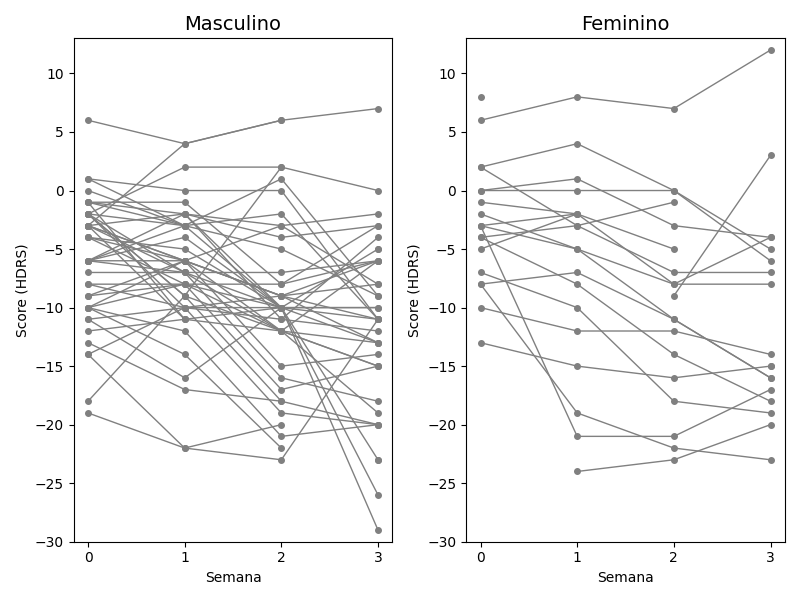
\includegraphics[width=0.7\linewidth]{imagens/secao1/perfis_individuais_por_sexo}
		}

\end{frame}


\begin{frame}{Gráfico de trajetórias individuais do Score HDRS  com perfil médio para cada sexo.}
	
	\centering
	\resizebox{0.8\textwidth}{!}{ % 
		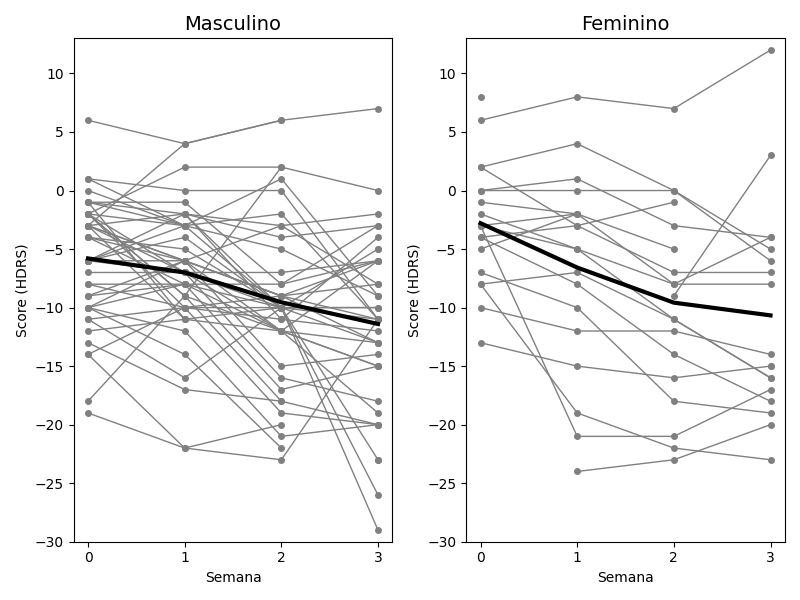
\includegraphics[width=0.7\linewidth]{imagens/secao1/perfis_individuais_por_sexo_com_perfil_medio}
	}
	
\end{frame}

\begin{frame}{Gráfico de trajetórias individuais do Score HDRS  com perfil médio e regressão para cada sexo.}
	
	\centering
	\resizebox{0.8\textwidth}{!}{ % 
		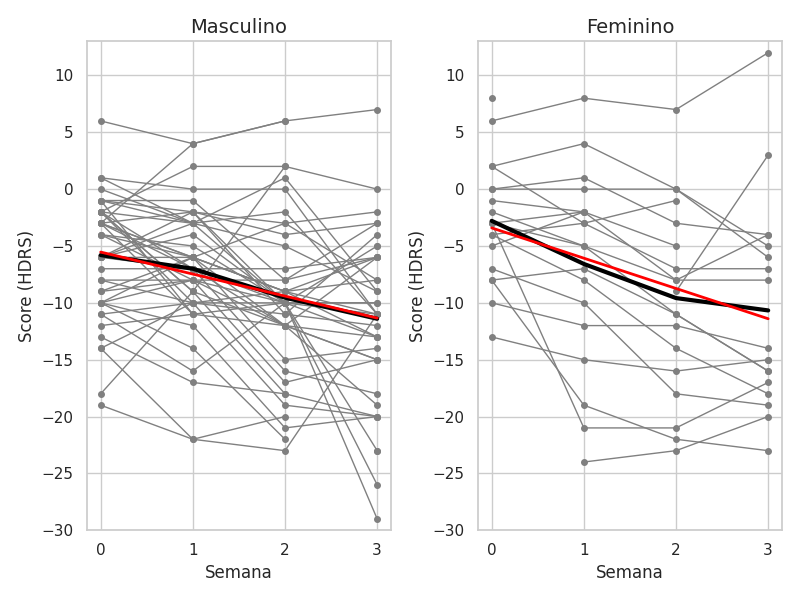
\includegraphics[width=0.7\linewidth]{imagens/secao1/perfis_individuais_por_sexo_com_perfil_medio_e_regressao}
	}
	
\end{frame}

\begin{frame}{Modelos de Regressão simples}
	\begin{block}{Modelo de Regressão para o sexo feminino}
		$$
		y = -3.41 - 2.66x + \varepsilon
		$$
	\end{block}
	\begin{block}{Modelo de Regressão para o sexo masculino}
		$$
		y = -5.53 - 1.93x + \varepsilon
		$$
	\end{block}
\end{frame}

\begin{frame}{}
	Gráfico de trajetórias individuais do Score HDRS para o sexo feminino com perfil médio e regressão simples e regressão polinomial do 2nd grau ajustada.
	\centering
	\resizebox{0.8\textwidth}{!}{ % 
		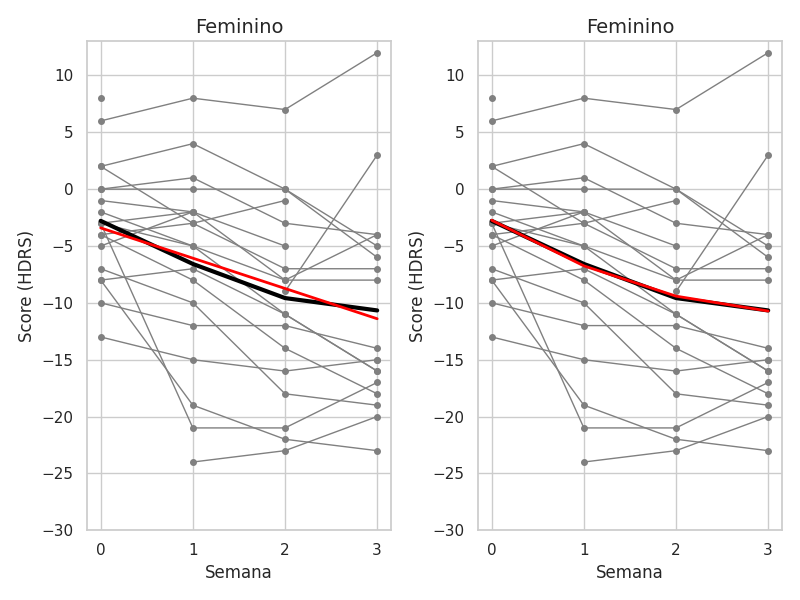
\includegraphics[width=0.7\linewidth]{imagens/secao1/perfis_individuais_por_sexo_com_perfil_medio_e_regressao_ajuste_polinomial}
	}
	
\end{frame}

\begin{frame}{}
	\centering
	\resizebox{\textwidth}{!}{ % 
		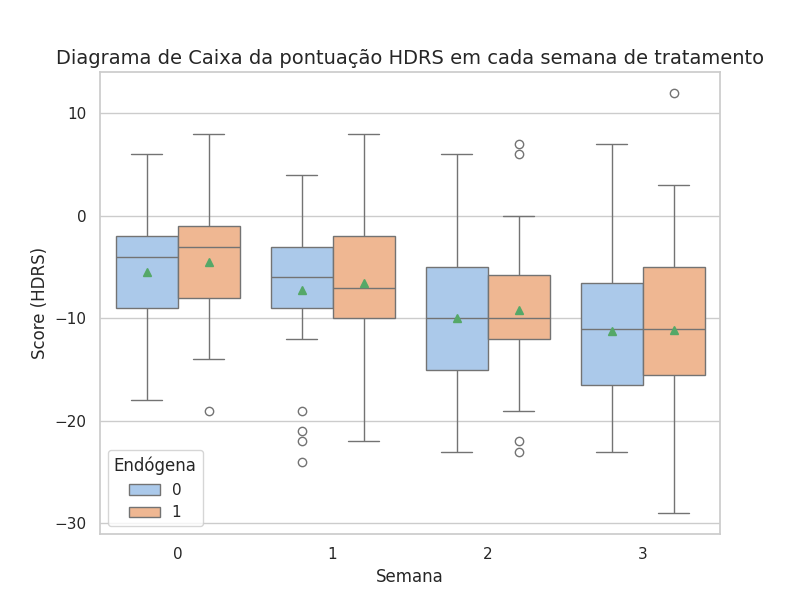
\includegraphics[width=0.7\linewidth]{imagens/secao1/diagrama_de_caixa_pontuacao_HDRS}
	}
	
\end{frame}


\begin{frame}{Regressão via Florestas Aleatórias}
	Para 4 árvores
	\centering
	\resizebox{\textwidth}{!}{ % 
		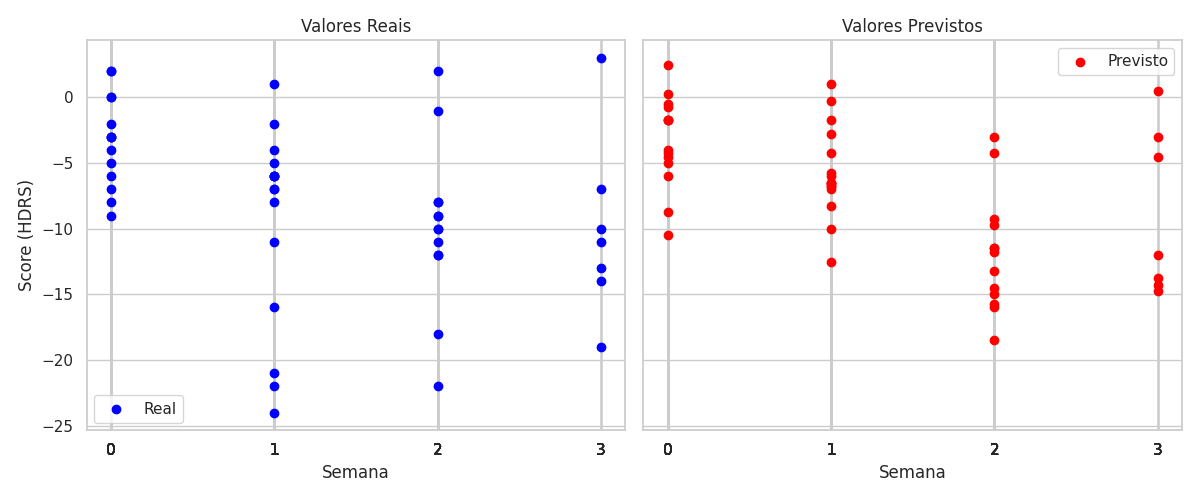
\includegraphics[width=0.8\linewidth]{imagens/secao1/RF_separados_4}
	}
	
\end{frame}

\begin{frame}{Regressão via Florestas Aleatórias}
	Para 10 árvores
	\centering
	\resizebox{\textwidth}{!}{ % 
		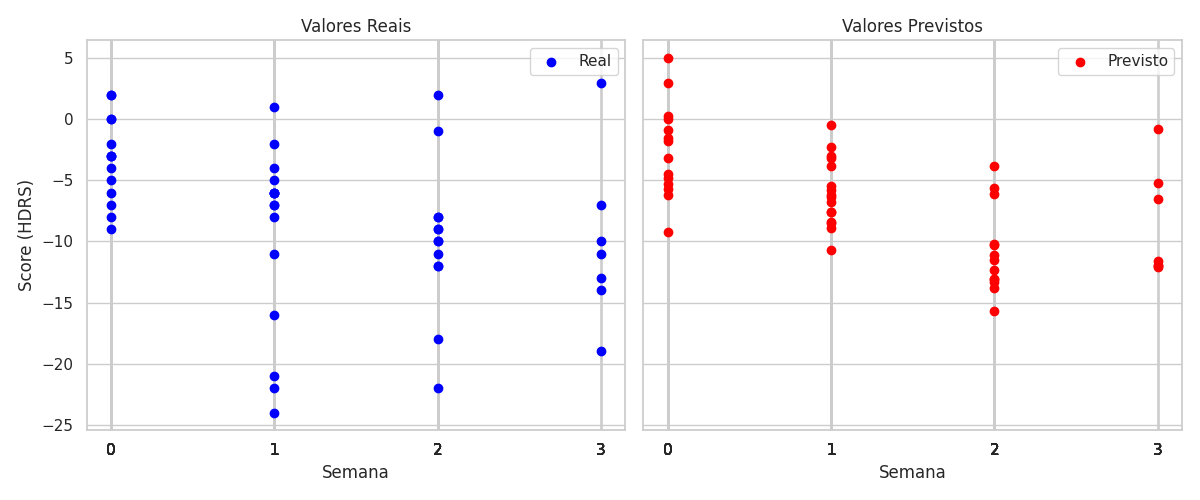
\includegraphics[width=0.8\linewidth]{imagens/secao1/RF_separados_10}
	}
	
\end{frame}

\begin{frame}{Regressão via Florestas Aleatórias}
	Para 50 árvores
	\centering
	\resizebox{\textwidth}{!}{ % 
		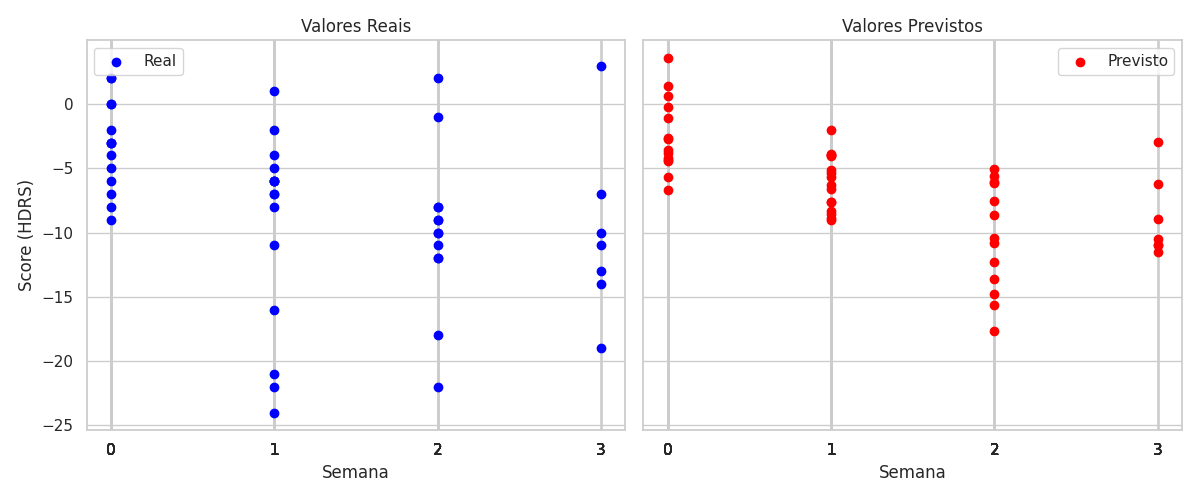
\includegraphics[width=0.8\linewidth]{imagens/secao1/RF_separados_50}
	}
	
\end{frame}

\begin{frame}{Regressão via Florestas Aleatórias}
	Para 100 árvores
	\centering
	\resizebox{\textwidth}{!}{ % 
		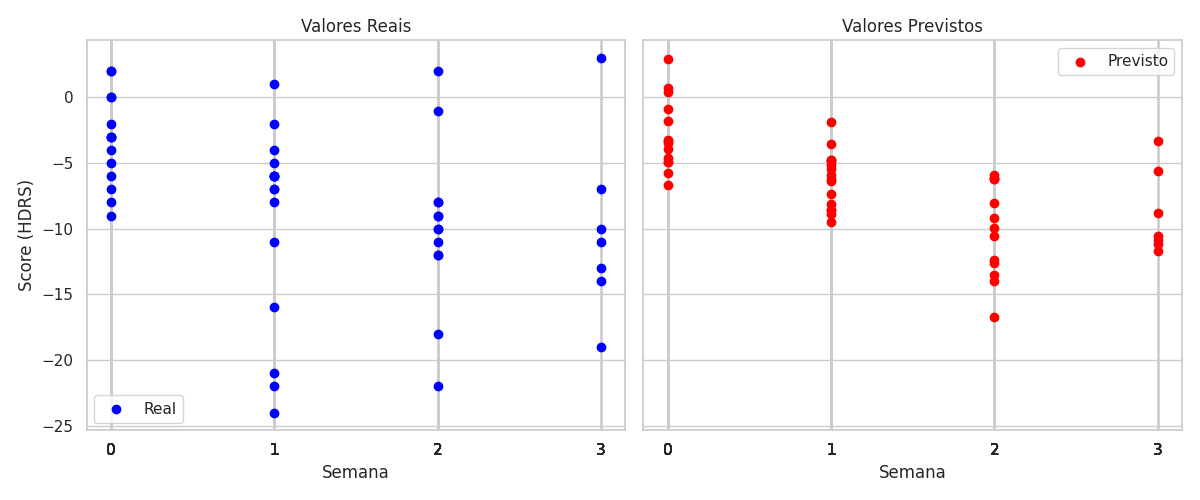
\includegraphics[width=0.8\linewidth]{imagens/secao1/RF_separados_100}
	}
	
\end{frame}

\begin{frame}{Melhor Escolha de Hiperparametro}
\begin{table}[h!]
	\centering
	\caption{Comparação de Hiperparâmetros do Random Forest}
	\begin{tabular}{|c|c|c|c|}
		\hline
		\textbf{Num de Árvores} & \textbf{EQM} & \textbf{$R^2$ Score} & \textbf{EMA} \\
		\hline
		4  & 44.06 & -0.0309 & 5.06 \\
		10 & 31.50 &  0.2630 & 4.33 \\
		50 & 33.30 &  0.2203 & 4.42 \\
		100 & 32.70 &  0.2300 & 4.27 \\
		\hline
	\end{tabular}
\end{table}

\end{frame}



\begin{frame}{Regressão via Florestas Aleatórias}
	\centering
	\resizebox{\linewidth}{!}{ % 
		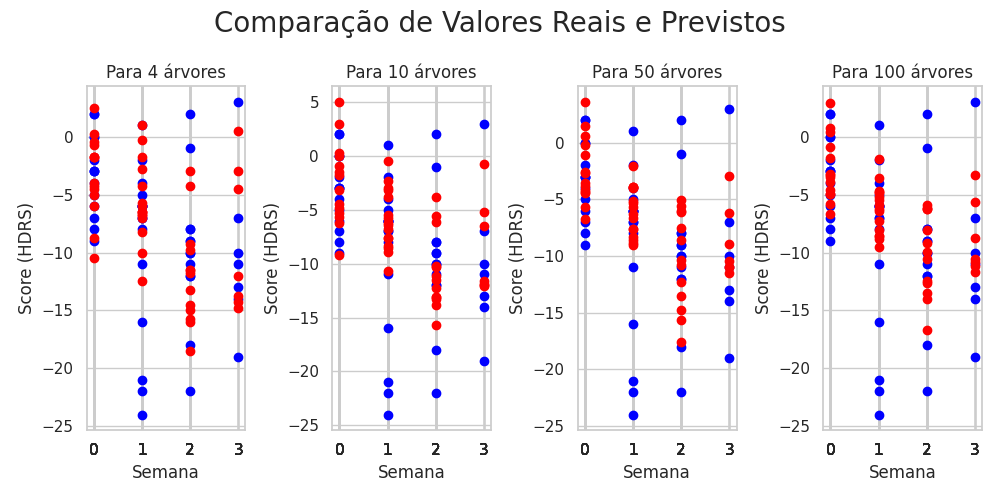
\includegraphics[width=0.6\linewidth]{imagens/secao1/RF_comparação}
	}
	
\end{frame}

\section{Seção I}
\begin{frame}{Explicações}
    % itemize
    Este é um template que pode ser utilizado para \nocite{Template_Beamer_UFC}:
    \begin{itemize}
        \item Apresentação de Trabalhos Acadêmicos
        \item Apresentação de Disciplinas
        \item Apresentações de Teses e Dissertações
    \end{itemize}

    \vspace{0.4cm} % vertical space
    
    % enumeration
    Para utilizar este template corretamente é importante que:
    \begin{enumerate}
        \item Tenha conhecimento mínimo sobre LaTeX
        \item Ler os comentários no template (explicações)
        \item Ler o README.md (documentação)
    \end{enumerate}

    \vspace{0.2cm}

    \example{Este é um texto de exemplo!} \emph{Texto de Ênfase!}
\end{frame}

%% ---------------------------------------------------------------------------
\subsection{Subseção I}
\begin{frame}{Criando Blocos}
    % Blocks styles
    \begin{block}{Bloco Padrão}
        Texto do corpo do bloco.
    \end{block}

    \begin{alertblock}{Bloco de Alerta}
        Texto do corpo do bloco.
    \end{alertblock}

    \begin{exampleblock}{Bloco de Exemplo}
        Texto do corpo do bloco.
    \end{exampleblock}   
\end{frame}

%% ---------------------------------------------------------------------------
\subsection{Subseção II}
\begin{frame}{Criando Caixas}
    \successbox{testando o success box}

    \pause

    \alertbox{testando o alert box}

    \pause

    \simplebox{testando o simple box}
\end{frame}

%% ---------------------------------------------------------------------------
\subsection{Subseção III}
\begin{frame}{Criando Algoritmos (Pseudocódigo)}
    \begin{algorithm}[H]
        \SetAlgoLined
        \LinesNumbered
        \SetKwInOut{Input}{input}
        \SetKwInOut{Output}{output}
        \Input{x: float, y: float}
        \Output{r: float}
        \While{True}{
          r = x + y\;
          \eIf{r >= 30}{
           ``O valor de $r$ é maior ou iqual a 10.''\;
           break\;
           }{
           ``O valor de $r$ = '', r\;
          }
         } 
         \caption{Algorithm Example}
    \end{algorithm}
\end{frame}

%% ---------------------------------------------------------------------------

\begin{frame}{Inserindo Algoritmos}
    \lstset{language=Python}
    \lstinputlisting[language=Python]{code/main.py}
\end{frame}

%% ---------------------------------------------------------------------------
\begin{frame}{Inserindo Algoritmos}
    \lstinputlisting[language=C]{code/source.c}
\end{frame}

%% ---------------------------------------------------------------------------
\begin{frame}{Inserindo Algoritmos}
    \lstinputlisting[language=Java]{code/helloworld.java}
\end{frame}

%% ---------------------------------------------------------------------------
\begin{frame}{Inserindo Algoritmos}
    \lstinputlisting[language=HTML]{code/index.html}
\end{frame}

%% ---------------------------------------------------------------------------
% This frame show an example to insert multicolumns
\section{Multicolunas}
\begin{frame}{Seção II - Multicolunas}
    \begin{columns}{}
        \begin{column}{0.5\textwidth}
            \justify
            É possível colocar mais de uma coluna utilizando os comandos de $\backslash$begin\{column\}\{\} e $\backslash$end\{column\}
        \end{column}
        \begin{column}{0.5\textwidth}
            \justify
            Porém, o espaçamento deve ser proporcional entre as colunas para que estas colunas não entrem em coflito. O espaçamento é dado pelo segundo argumento do $\backslash$begin.
        \end{column}
    \end{columns}    
\end{frame}

%% ---------------------------------------------------------------------------
% This frame show an example to insert figures
\section{Imagens}
\begin{frame}{Seção III - Figures}
    \begin{figure}
        \centering
        \caption{Emblema da UFC.}
        
\includegraphics[scale=0.3]{libs/emblemufc.pdf}
        \source{Obtido pelo site oficial da UFC \cite{siteufc} \cite{einstein}}
        \label{fig:ufc_emblem}
    \end{figure}
\end{frame}

%% ---------------------------------------------------------------------------
% Reference frames
\begin{frame}[allowframebreaks]
    \frametitle{Referências}
    \printbibliography
\end{frame}

%% ---------------------------------------------------------------------------
% Final frame
\begin{frame}{}
    \centering
    \huge{\textbf{\example{Obrigado!!!}}}
    
    \vspace{1cm}
    
    \Large{\textbf{Contato:}}
    \newline
    \vspace*{0.5cm}
    \large{\email{cicero.hitzschky@alu.ufc.br}}
\end{frame}

\end{document}